
\subsection{Aircraft force diagram}
The aircraft in question is the EcoSoar; a flying wing.
It has two control surfaces, one on each wing called elevons.
In front of each wing a motor and propeller is mounted providing thrust.
The motors also supply an airflow over the control surfaces when the aircraft is not moving through the air.


\begin{figure}[h]
    \center
    \begin{tikzpicture}
    \begin{tikzpicture}
    \begin{scope}[shift={(6,2.4)}]
    % Coord sys.
    \begin{scope}[shift={(1.2,-0.1)}]
        \draw[thick, ->] (-6,2) -- (-6,2.5) node[anchor=south east]{$x$};
        \draw[thick, ->] (-6,2) -- (-5.5,2) node[anchor=south west]{$y$};
        \draw[] (-6,2) circle (0.15cm);
        \draw[] (-6.1,1.9) -- (-5.9,2.1);
        \draw[] (-6.1, 2.1) -- (-5.9,1.9);
        \node[] at (-6.3,1.9) {$z$};
    \end{scope}

    % main body
    \draw (0,0) rectangle (1,2);
    % left wing
    \draw (0,2) -- (-5,0) -- (-5,-1) -- (0,0);
    % right wing
    \draw (1,2) -- (6,0) -- (6,-1) -- (1,0);
    % winglets, left and right
    \draw[very thick] (6,0) -- (6,-1);
    \draw[very thick] (-5,0) -- (-5,-1);

    % wingspan
    \draw[<->, thin] (-5,-2.2) -- (6, -2.2);
    \draw[dotted] (-5,-1) -- (-5, -2.5);
    \draw[dotted] (6, -1) -- (6, -2.5);
    \node at (0.5,-2.4) {$b$};

    % right Winglet forces
    \draw[fill=black] (6,-0.5) circle (0.05cm) ;
    \draw[->, thick] (6,-0.5) -- (6.5, -0.5);
    \node[] at (6.7,-0.8) {$L_{W_R}$};
    \draw[dotted] (6,-0.5) -- (7.2,-0.5);
    \draw[very thin, <->] (6.7,-0.5) -- (6.7, 1.4);
    \node[] at (7, 0.4) {$x_W$};

    \draw[->, thick] (6,-0.5) -- (6, -1.5);
    \node[] at (6.5,-1.5) {$D_{W_R}$};

    %left and right flaps
    %\draw (-4.4,-0.88) circle (0.1cm);
    %\draw (-1, -0.2) circle (0.1cm);
    \draw (-4.4, -0.88) -- (-4.4, -0.5) -- (-1, 0.25) -- (-1, -0.2);
    \draw (5.4, -0.88) --  (5.4, -0.5) -- (2, 0.25) -- (2,-0.2);

    % left and right propellers
    \draw[thick, ->] (-2.5,1) -- (-2.5,2) node[anchor=south east]{$T_L$};
    \draw[thick, ->] (3.5,1) -- (3.5, 2) node[anchor=south west]{$T_R$};

    % prop distance to cg
    \draw[<->] (-2.5, 2.5) -- (0.5, 2.5);
    \node[] at (-1, 2.7) {$y_T$};
    \draw[dotted] (3.5,2) -- (4.5,2);
    \draw[<->] (4.5,2) -- (4.5,1.4);
    \node[] at (4.8, 1.7) {$x_T$};

    % propeller cone. Left then Right
    \draw[dotted] (-3,2) -- (-3,-1);
    \draw[dotted] (-2,2) -- (-2,-1);
    \draw[dotted] (4,2) -- (4,-1);
    \draw[dotted] (3,2) -- (3,-1);

    % Propeller cone width
    \draw[<->] (4,-1) -- (3,-1);
    \node[] at (3.5, -1.2) {$y_w$};

    % Surface area aileron
    \node[] at (-2.5, -0.3) {$S_{a_w}$};
    \node[] at (-3.6, -0.53) {$S_a$};
    \node[] at (-1.6, -0.1) {$S_a$};

    % Wind surface areas
    \node[] at (2,0.8) {$S_w$};
    \node[] at (5,0) {$S_w$};
    \node[] at (3.35,0.85) {$S_{w_w}$};

    % Lift force, left
    \draw (-2.2, 0.4) circle (0.2cm);
    \draw[fill=black] (-2.2, 0.4) circle (0.025cm);
    \node[] at (-1.7, 0.4) {$L_L$};

    % Lift force, right
    \draw (3.2, 0.4) circle (0.2cm);
    \draw[fill=black] (3.2, 0.4) circle (0.025cm);
    \draw[dotted] (3.2, 0.4) -- (6.5,0.4);
    \node[] at (2.7, 0.4) {$L_R$};

    % Drag force, right
    \draw[->] (3.2,0.4) -- (3.2, -0.3);
    \node[] at (3.5,-0.3) {$D_R$};

    % Lift force distance
    \draw[<->] (0.5, -0.7) -- (3.2, -0.7);
    \node[] at (2, -0.5) {$y_{ac}$};
    % Right x distance
    \draw[<->] (6.2,1.4) -- (6.2, 0.4);
    \node[] at (5.8, 0.9) {$x_{ac}$};

    % Aileron force
    \draw (-2.5, -0.9) circle (0.2cm);
    \draw[] (-2.35, -0.75) -- (-2.65,-1.05);
    \draw[] (-2.65, -0.75) -- (-2.35, -1.05);
    %\node[] at (-2.4, -1.3) {$F_L$, $F_{L_T}$};
    \node[] at (-1.5, -1.0) {$F_L$, $F_{L_T}$};
    \draw[dotted] (-2.5, -0.9) -- (-5.5, -0.9);
    % Aileron drag
    \draw[->, thick] (-2.5, -0.9) -- (-2.5, -1.5);
    \node[] at (-1.4, -1.4) {$D_{a_L}$, $D_{a_{L,T}}$};

    % Distance flap force
    \draw[<->] (0.5,-1.8) -- (-2.5, -1.8);
    \node[] at (-1, -2) {$y_f$};
    \draw[<->] (-5.3, 1.4) -- (-5.3, -0.9);
    \node[] at (-5.6, 0.2) {$x_f$};

    % Center of Grav.
    \draw[fill=black] (0.5, 1.4) circle (0.1cm);
    \draw[dotted] (0.5,1.4) -- (0.5,-2);
    \draw[dotted] (0.5,1.4) -- (7.1,1.4);
    \draw[dotted] (0.5,1.4) -- (-5.5,1.4);
    \node[] at (0.55, 1.1) {c.g.};


    %mark 0,0
    %\draw (0,0) circle (0.1cm);

\end{scope}
\end{tikzpicture}
    \end{tikzpicture}
    \caption{Drawing of the EcoSoar, its propellers with wake and its control surfaces in body frame.}
    \label{airplane}
\end{figure}

The elevon forces, $F_L$, $F_{L_T}$, $D_{a_{L}}$ and $D_{a_{L,T}}$, have only been marked on the left wing, but exist symmetrically on the right wing with index $R$ instead of $L$.
The same is true for the drag force, $D_R$ and the winglet forces, $L_{W_R}$ and $D_{W_R}$, existing symmetrically on the left side.
$F_L$ is the force due to elevon deflection over surface area $S_a$, and $F_{L_T}$ is the force due to elevon deflection over $S_{a_w}$; the surface in the wake of the propeller.
Similarly for the drag, $D_{\alpha_L}$, $D_{\alpha_{L,T}}$, forces.
We also split the wing area into two sections: $S_w$ for the wing area outside the wake, and $S_{w_w}$ for the wing area in the wake.
The thrust forces, $T_i$, are assumed to act at the arrow end of the vector due to the offset in $x$ created by the motor and drive shaft.
The lift forces, $L_L$ and $L_R$, are functions of airflow over wing outside of wake and in the wake, which in turn are functions of aircraft velocity, propeller speed, angle of attack, air density, wing shape, etc.



\subsubsection{Aerodynamic Lift force}

The lift force of a wing depends on several factors.
Mainly: geometrical shape, dynamic pressure and angle of attack.
The bigger the wing the more lift.
The faster air flows the more lift.
The further away from hitting the wing straight on, usually more lift.

Important note: Lift is defined as the \textbf{Aerodynamic force component perpendicular to the incoming airflow.} This means that, for example, the lift force labeled in figure \ref {airplane} as \textbf{$L_L$ is not the aerodynamic lift but rather the lift force in body frame.} The same argument applies to the drag forces.

Aerodynamic lift is usually modeled as:
\begin{equation}
    L = Q  C_L S
\end{equation}
where $S$ is a reference surface area of the wing and $Q$ is the dynamic pressure:
\begin{equation}
    Q = \frac{1}{2} \rho v^2
\end{equation}
$\rho$ is the density of air and $v$ the velocity of the air hitting the wing.
$C_L$ is the coefficient of lift, a function of the angle of attack.
This coefficient is not linear. Empirical studies have found functions similair to the one in figure \ref{clalpha}.
\begin{figure}[h]
    \center
    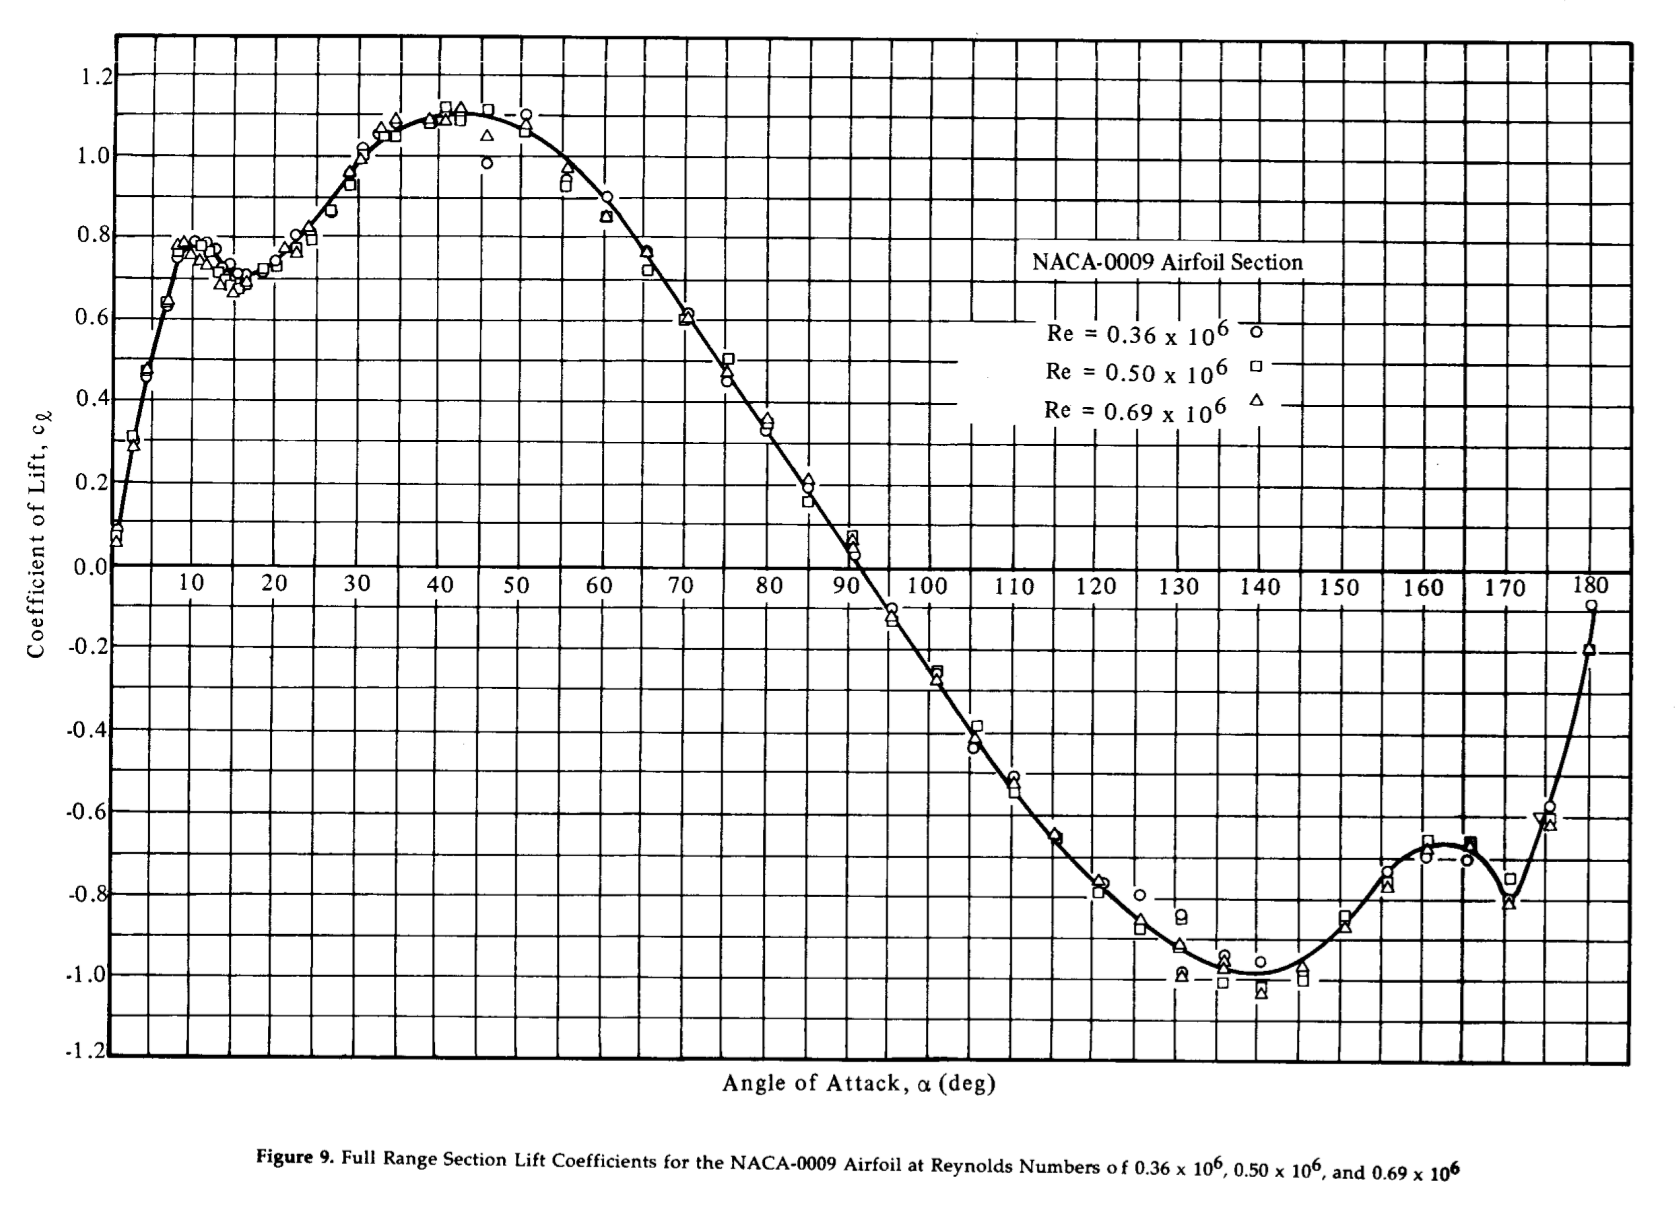
\includegraphics[scale=0.15]{aoa_80s.png}
    \caption{Coefficient of lift for a symmetrical wing vs angle of attack for the entire 180 degree rotation of the wing. The function is periodic.}
    \label{clalpha}
\end{figure}

The angle of attack, $\alpha$, is formally the angle at which the air is hitting the wing relative the body frame x-z axis.
If air is aligned with the $x$-axis $\alpha$ is zero, and if aligned with the $z$-axis $\alpha$ is 90.
(The airflow will obviously be in the negative axis direction since the airplane is flying in the positive direction and hitting the air).
Thus, if we assume no wind the angle of attack is only dependent on the aircraft velocity $\bar{v}$.
Normally this is modeled as:
\begin{equation}
    \alpha = tan^{-1}(\frac{v_z}{v_x})
    \label{eq:aoa}
\end{equation}
but in our case the velocity may have any direction in the $x$-$z$ plane, and is not limited to the right half plane.
The polar coordinates for vector $\bar{v}$ in the figure below, figure \ref{polar}, are:
\begin{equation}\begin{split}
    v_x =& \, r \, cos(\alpha) \\
    v_y =& \, r \, sin(\alpha) \\
    r =& \sqrt{v_x^2 + v_z^2}
    \label{eq:polar}
\end{split}\end{equation}
where $\alpha$ is in the interval $[-\pi,\pi]$.

\begin{figure}[h]
    \center
    \begin{tikzpicture}
    
    \draw[->] (-2,0) -- (2,0); % x-axis
    \node[] (x) at (2,-0.2) {$v_x$};
    \draw [->](0,-1) -- (0,2); % y-axis
    \node[] (y) at (0.3,2) {$v_z$};

    % Vector
    \draw[->, thick] (0:0) -- (90+45:1.5);
    \node[] at (90+45:1.7) {$\bar{v}$};

    % help lines
    \draw[dotted] (-1.05,0) -- (90+45:1.5);
    \draw[dotted] (0,1.05) -- (90+45:1.5);

    % angle
    \draw[->] (0.3,0) arc(0:45+90:0.3);
    \node[] at (0.3,0.4) {$\alpha$};
\end{tikzpicture}
    \caption{Velocity vector $\bar{v}$ in polar coordinates.}
    \label{polar}
\end{figure}

\subsubsection{Aerodynamic drag}
Similarly to aerodynamic lift the wing will also have an aerodynamic drag force, but parallel to the incoming flow and not perpendicular as lift.
The drag is also modeled like so:
\begin{equation}
    D = Q C_D S
\end{equation}
where the coefficient of drag, $C_D$, can also be experimentally obtained as in figure \ref{drag}.

\begin{figure}[h]
    \center
    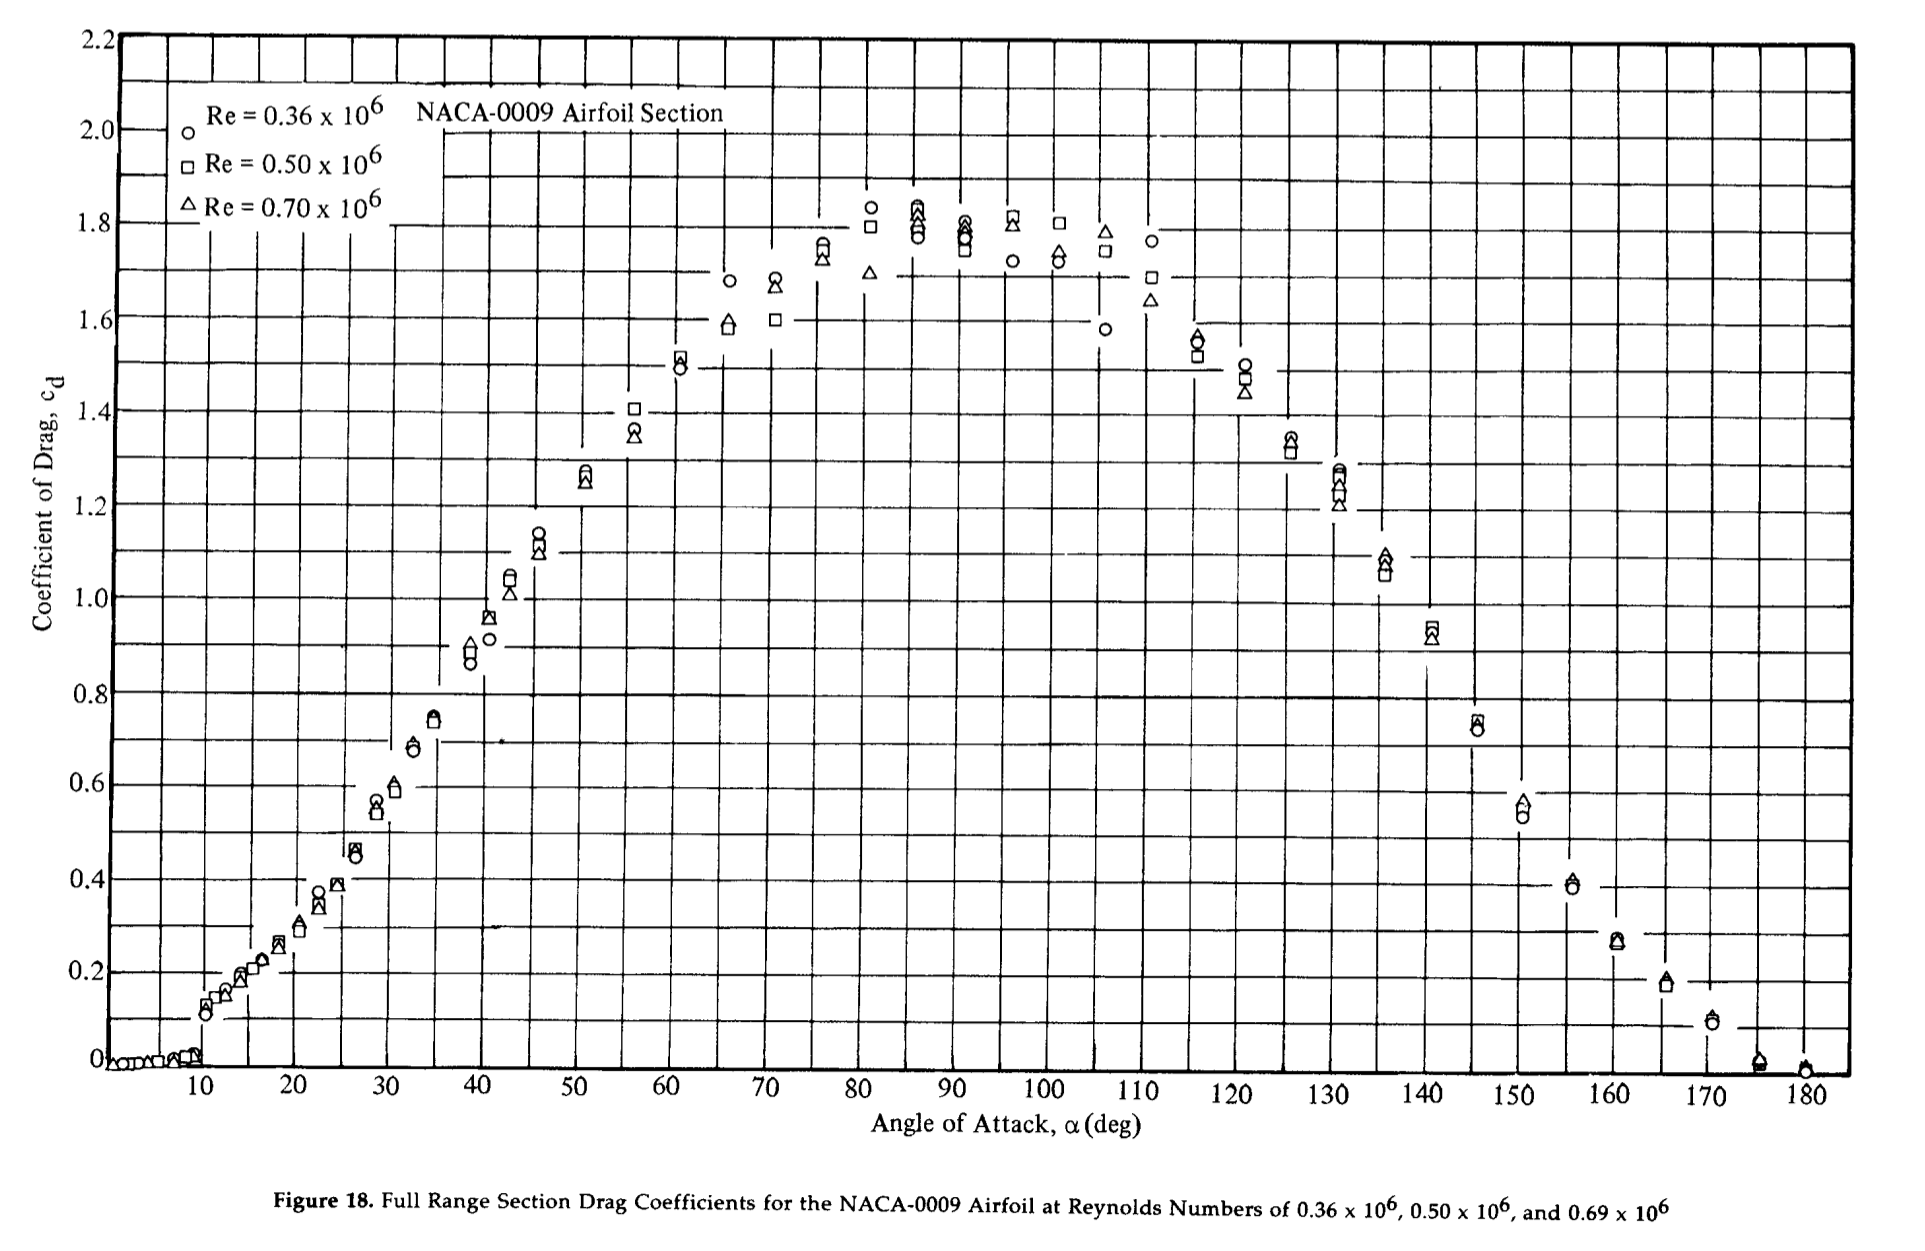
\includegraphics[scale=0.15]{drag180.png}
    \caption{Coefficient of drag for a symmetrical wing vs angle of attack for the entire 180 degree rotation of the wing.}
    \label{drag}
\end{figure}


\subsubsection{Lift and drag in body frame}

Since the aerodynamic lift and drag forces are relative the incoming airflow, i.e. functions of the angle of attack, $\alpha$, the body frame Lift and Drag have to transformed:
\begin{equation}\begin{split}
    L_i &= cos(\alpha) L + sin(\alpha) D \\
    D_i &= -sin(\alpha) L + cos(\alpha) D
    \label{LDbodyframe}
\end{split}\end{equation}
Note that the above forces are in the direction labeled in figure \ref{airplane} and not necessarily in the positive axis they act in.
From equation \ref{eq:polar} we see that
\begin{equation}\begin{split}
    v_x =& \, r \, cos(\alpha) \Rightarrow cos(\alpha) = \frac{v_x}{\sqrt{v_x^2 + v_z^2}} \\
    v_z =& \, r \, sin(\alpha) \Rightarrow sin(\alpha) = \frac{v_z}{\sqrt{v_x^2 + v_z^2}}
\end{split}\end{equation}
If we substitute in expressions for aerodynamic lift and drag we obtain:
\begin{equation}\begin{split}
    L_i =&  \frac{v_x}{\sqrt{v_x^2 + v_z^2}} Q C_L S +
            \frac{v_z}{\sqrt{v_x^2 + v_z^2}} Q C_D S \\
    D_i =& -\frac{v_z}{\sqrt{v_x^2 + v_z^2}} Q C_L S +
            \frac{v_x}{\sqrt{v_x^2 + v_z^2}} Q C_D S \\          
\end{split}\end{equation}
which simplify into:
\begin{equation}\begin{split}
    L_i =& 
     S \frac{1}{2} \rho v^2 \left( \frac{C_L v_x + C_D v_z}{\sqrt{v_x^2 + v_z^2}} \right) \\
     %
    D_i =& 
     S \frac{1}{2} \rho v^2 \left( \frac{-C_L v_z + C_D v_x}{\sqrt{v_x^2 + v_z^2}} \right)
     \label{liftdragbody}
\end{split}\end{equation}
where $v = \sqrt{v_x^2 + v_y^2 + v_z^2}$.


\subsection{Moment due to force}

Any force not acting at the center of gravity will produce a moment around c.g.
The moment of a force is:
\begin{equation}
    \bar{M} = \bar{r} \times \bar{F}
\end{equation}
With our assumptions the above equation can be written as:
\begin{equation}
    \bar{M} = (r_x, r_y, 0) \times (F_x, F_y, F_z) = 
    \left[ \begin{matrix}
    F_z r_y \\
    -F_z r_x \\
    F_y r_x - F_x r_y \end{matrix} \right]
\end{equation}

\subsubsection{Pitching moment}
Lift due to camber on a wing acts at ~50\% of the cord line.
Lift due to angle of attack acts at roughly 25\% of the cord line.
This makes the force acting point, center of pressure, move along the cord line when angle of attack and aircraft velocity changes.
A common simplification is to choose the aerodynamic center, a.c., as the point at which Lift acts.
It can be shown that placing the a.c. at the 25\% cord position 
makes the moment generated vary little as angle of attack changes, yielding simpler equations.
The pitching moment due to lift can now be expressed as:
\begin{equation}
    \tau_{y,lift} = \sum_{j \in [w, w_w]}
    C_{m,y,l} Q S_j l +  \cancelto{0}{\sum_{j \in [w, w_w]}
    C_{m,y,l,\alpha} Q S_j l \alpha}
\end{equation}
where $l$ is the characteristic length of the wing, usually taken as the mean cord for pitching moments and the wingspan for rolling and yawing moments.

\subsection{Equations of motion}

The equations of motion can be split into three parts: one part due to gravity, one part due to the rigid body frame being an accelerated reference frame, and one part due to aerodynamic forces.

\subsubsection{Attitude}
The attitude is represented by a quaternion:
\begin{equation}
\bar{q} = [q_0, q_1, q_2, q_3]^T
\end{equation}
Any vector, $\bar{r}_w$, in world frame can be represented in the body frame by the conversion:
\begin{equation}
    \bar{r}_b = \bar{q} \bar{r}_w \bar{q^*}
\end{equation}
\subsubsection{Gravity}
In the case of gravity, $\left[\begin{smallmatrix}0\\0\\mg\end{smallmatrix}\right]_w$, the force, $m \bar{g}$, becomes
\begin{equation}
m \dot{\bar{v}}_b = \left[ \begin{matrix}
    2 (\bar{q_1} \bar{q_3} + \bar{q_0} \bar{q_2})  \\
    2 (\bar{q_2} \bar{q_3} - \bar{q_0} \bar{q_1})  \\
    (\bar{q_0}^2 - \bar{q_1}^2 - \bar{q_2}^2 + \bar{q_3}^2) 
    \end{matrix} \right] m g
\end{equation}
Gravity acts in the center of gravity and creates no moment.
Since gravity is in world frame and we want to express it in body frame we need to conjugate the quaternion.